\documentclass[11pt]{article}
\usepackage{latexsym}
\usepackage{amsmath}
\usepackage{listings}[language=Python]
\usepackage{amssymb}
\usepackage{amsthm}
\usepackage{epsfig}
\usepackage[tight]{subfigure}
\usepackage{color}
\usepackage{listings}
\usepackage{setspace}
\definecolor{Code}{rgb}{0,0,0}
\definecolor{Decorators}{rgb}{0.5,0.5,0.5}
\definecolor{Numbers}{rgb}{0.5,0,0}
\definecolor{MatchingBrackets}{rgb}{0.25,0.5,0.5}
\definecolor{Keywords}{rgb}{0,0,1}
\definecolor{self}{rgb}{0,0,0}
\definecolor{Strings}{rgb}{0,0.63,0}
\definecolor{Comments}{rgb}{0,0.63,1}
\definecolor{Backquotes}{rgb}{0,0,0}
\definecolor{Classname}{rgb}{0,0,0}
\definecolor{FunctionName}{rgb}{0,0,0}
\definecolor{Operators}{rgb}{0,0,0}
\definecolor{Background}{rgb}{0.98,0.98,0.98}
\lstdefinelanguage{Python}{
numbers=left,
numberstyle=\footnotesize,
numbersep=1em,
xleftmargin=1em,
framextopmargin=2em,
framexbottommargin=2em,
showspaces=false,
showtabs=false,
showstringspaces=false,
frame=l,
tabsize=4,
% Basic
basicstyle=\ttfamily\small\setstretch{1},
backgroundcolor=\color{Background},
% Comments
commentstyle=\color{Comments}\slshape,
% Strings
stringstyle=\color{Strings},
morecomment=[s][\color{Strings}]{"""}{"""},
morecomment=[s][\color{Strings}]{'''}{'''},
% keywords
morekeywords={import,from,class,def,for,while,if,is,in,elif,else,not,and,or,print,break,continue,return,True,False,None,access,as,,del,except,exec,finally,global,import,lambda,pass,print,raise,try,assert},
keywordstyle={\color{Keywords}\bfseries},
% additional keywords
morekeywords={[2]@invariant,pylab,numpy,np,scipy},
keywordstyle={[2]\color{Decorators}\slshape},
emph={self},
emphstyle={\color{self}\slshape},
%
}
\linespread{1.3}


\newcommand\X{\mathcal{X}}
\newcommand\Y{\mathcal{Y}}
\newcommand\HH{\mathcal{H}}

\DeclareMathOperator*{\minimize}{min}
\DeclareMathOperator*{\maximize}{max}

\usepackage{algorithm}
 %on linux you may need to run sudo apt-get install texlive-full to install algorithm.sys
\usepackage{algorithmic}

\usepackage{verbatim}

\newcommand{\handout}[5]{
  \noindent
  \begin{center}
  \framebox{
    \vbox{
      \hbox to 5.78in { {#1} \hfill #2 }
      \vspace{4mm}
      \hbox to 5.78in { {\Large \hfill #5  \hfill} }
      \vspace{2mm}
      \hbox to 5.78in { {\em #3 \hfill #4} }
    }
  }
  \end{center}
  \vspace*{4mm}
}

\newcommand{\lecture}[5]{\handout{#1}{#2}{#3}{#4}{#5}}
\newcommand{\collision}[0]{\mathrm{collision}}
\newcommand{\nocollision}[0]{\overline{\collision}}

\newcommand*{\QED}{\hfill\ensuremath{\square}}

\newtheorem{theorem}{Theorem}
\newtheorem{corollary}[theorem]{Corollary}
\newtheorem{lemma}[theorem]{Lemma}
\newtheorem{observation}[theorem]{Observation}
\newtheorem{proposition}[theorem]{Proposition}
\newtheorem{definition}[theorem]{Definition}
\newtheorem{claim}[theorem]{Claim}
\newtheorem{fact}[theorem]{Fact}
\newtheorem{assumption}[theorem]{Assumption}
\newtheorem{note}[theorem]{Note}

% 1-inch margins, from fullpage.sty by H.Partl, Version 2, Dec. 15, 1988.
\topmargin 0pt
\advance \topmargin by -\headheight
\advance \topmargin by -\headsep
\textheight 8.9in
\oddsidemargin 0pt
\evensidemargin \oddsidemargin
\marginparwidth 0.5in
\textwidth 6.5in

\parindent 0in
\parskip 1.5ex
%\renewcommand{\baselinestretch}{1.25}

\begin{document}

\lecture{Statistical Techniques in Robotics (16-831, S20)}{Lecture \#1
  (Wednesday, February 3)}{Lecturer: Kris Kitani}{Scribes:  Manikandtan Chiral Kunjunni Kartha, Erica Weng}{PWEA, Greedy / Consistent Algorithm}
\
%This section serves as a review of the previous lecture and any other context required to frame the content of the current lecture. 

%You may format the scribes in any way you like, aside from changing font style, size and page format. Please use subsections and paragraphs to increase the readability of your notes.

%Length requirement 1-2 pages.
\section{Recap}
In the previous lecture we discussed about the different kinds of robot learning problems and how the differ. Based on the properties of feedback a robot receives from the environment, we can classify the learning algorithms as following \cite{littman2015reinforcement}:
\begin{enumerate}
\item Exhaustive (robot is exposed to all possible variations of the data) vs Sampled (exposed to only a subset of the variations)
\item Evaluative (the robot receives no feedback about possible alternative actions) vs Instructive (the robot receives the score for all possible actions)
\item Sequence (whether the outcome of a current action affects the next action) vs One-shot (outcome of current action doesn’t affect the next action)
\end{enumerate}
Most robot learning techniques like Reinforcement learning suffer from generally weak feedback (evaluative and sequential) as compared to other machine learning techniques like supervised learning and is hence generally harder to solve.

To understand these these properties, we looked at a few common learning techniques and where they lie in the spectrum of feedback properties(See Figure \ref{fig:learning_prob}).
\begin{itemize}
    \item Reinforcement Learning: say in the case of autonomous driving, the system initiates actions which influence later states (sequential) and the system does not receive feedback on each possible action it could have taken at a given time step(evaluative) as well as sampled.
    \item Tabular Reinforcement Learning : say in a \textit{Gridworld} problem, while the current actions influence later states(sequential), the system does receive feedback on each possible action for a state(instructive) and can be exhaustive for small enough problems. The presence of strong instructive and exhaustive feedback helps in designing really efficient algorithms like \textit{Dijkstra's} to solve such problems. 
    \item Multi Armed Bandit: in a bandit system where the reward distribution in not dynamic(rigged), the problem is one-shot, exhaustive and evaluative.
\end{itemize}


\begin{figure}[ht]
    \centering
    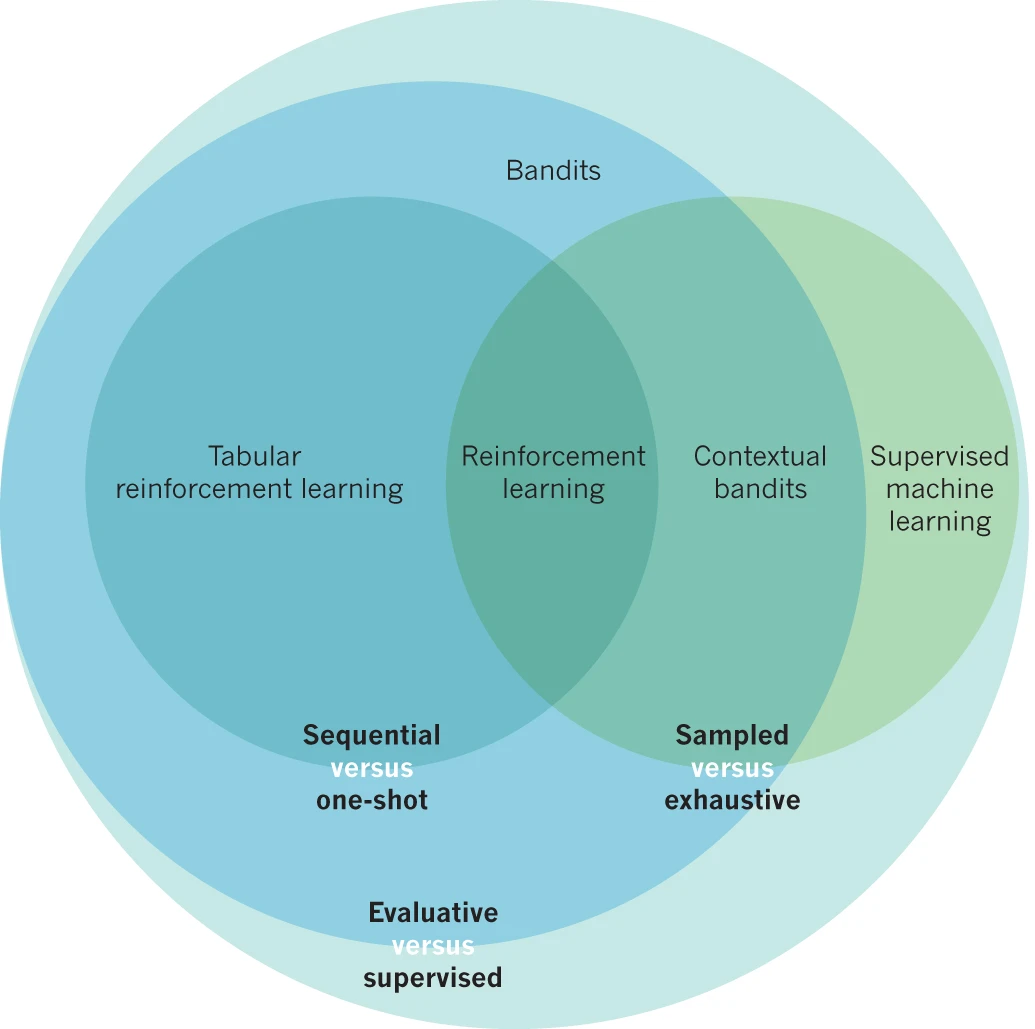
\includegraphics[width=0.6\textwidth]{Littman.png}
    \caption{Three kinds of feedback in machine learning and examples of learning problems that result from their combination. \cite{littman2015reinforcement}}
    \label{fig:learning_prob}
\end{figure}

\section{Online Learning vs. Supervised Learning}
The core idea behind online learning is the fact that algorithms makes predictions and learns with each sample input as it is received. In its simplest form the input data is assumed to be one-shot (there is no correlation between samples). However, the feedback maybe instructive or evaluative and exhaustive or sampled. The goal of the online learner is to minimize the loss (when system is realizable – the learner has access to the perfect hypothesis) or more generally – to minimize the regret. 

Supervised Learning has clearly separate train and test stages – and follows the assumption that the data observed during training is representative of the data which will be observed during test stage.
Online Learning does away this separation and performs incremental learning over each received input. This helps the system adapt in situations where the data distribution received is stochastic or adversarial, something which supervised learning would have trouble with. Online learning technique may also be a better strategy when the training dataset is too large to either fit in memory or be processed at the same time. Interestingly the supervised learning method of Stochastic Gradient Descent (SGD) when trained with a batch size of one may be seen as an online learning technique during its training phase.  

\section{Prediction With Expert Advice (PWEA)}
PWEA is a method of online learning where the system takes decisions based on advice from a set of experts and over time with the goal to be as good as possible as the best expert in the group, if not better. Over time the system learns from making mistakes based on the advice from each expert and updates the hypothesis function which modifies the weighting given to each expert in the group.  The different way to choose your hypothesis function and weight update strategy gives us different variations of PWEA.\cite{Bianchi1997Expert,Bianchi1999sequences}

\subsection{Realizability}

\definition{\normalfont\textbf{Realizability} is the assumption that the learner has access to the perfect hypothesis.}

\normalfont
Realizability is an assumption made about the hypothesis space that the learner can achieve at least one perfect hypothesis which will give the global optima for the loss function. Under the conditions of realizability, the performance is measured in terms of the mistake bound, which represents, in retrospect, the cost for not following the perfect hypothesis. In a realistic scenario this may not always be possible and in later methods we would relax this realizability assumption and allow even the best expert to make a few mistakes. In a system of imperfect experts(non-realizability), we will evaluate the performance of the algorithm in terms of the \textit{regret bound} instead of the \textit{mistake bound}. In such a case, we would like to design algorithms which can minimize regrets.

\section{Greedy / Consistent Algorithm}
With the Greedy/Consistent algorithm, the system uses a learning rule where it picks the first expert in its pool of experts (Greedy) who has been consistently correct in its predictions up until now, and bases its decision solely based on that expert. With each mistake made, the pool of consistent experts reduces by at least 1. Assuming a realizable system where there is at least one perfect expert, the system will be as good as the consistent expert.

There are multiple issues with this strategy, the most obvious one being if realizability is not met, the algorithm will no longer have a pool of experts to pick from and will terminate. The fact that algorithm requires strict consistency also may eliminate an expert who is reasonably good but not perfect if the expert makes a mistake at an early timestep.

Now we define our problem space formally: we have the instance domain $\X$, or the set of possible observations that can be seen any timestep $t$; the target domain $\Y$, or the set of possible outcomes that can occur; and the hypothesis class $\HH = \{h: \X \rightarrow \Y \}$, a series of functions mapping an element in the instance domain to an element in the target domain, each of which determines how we will make a prediction based on the observations we see. The Version space $\mathbf{V}^{(t)}$ at time $t$ is defined as the set of experts whom we still trust at time $t$; all experts in the version space at time $t$ have not yet made a mistake. Then, the Greedy Algorithm pseudocode is listed in algorithm \ref{algo:greedy}.

\begin{algorithm}[H]
\caption{Greedy / Consistent Algorithm}
\label{algo:greedy}
\begin{algorithmic}[1]
\STATE $\mathbf{V^{(1)}} = \mathcal{H}$  \hfill $\triangleright$ Version space initially stores all hypotheses
\FOR{$t=1,\;\cdots,\;T$}
\STATE \textsc{Receive} ($\textbf{x}^{(t)}$) \hfill $\triangleright$ Receive expert prediction
\STATE $h =\textsc{FirstElem}(\textbf{V}^{(t)}) \hfill \triangleright$ Greedy selection 
\STATE $\hat{y}^{(t)} = h(\mathbf{x}^{(t)})$ \hfill $\triangleright$ predict using first expert in remaining list of experts
\STATE \textsc{Receive} ($y^{(t)}$) \hfill $\triangleright$ Receive true outcome
\STATE $\mathbf{V}^{(t+1)}\leftarrow \{ h \in \mathbf{V}^{(t)} : h(\textbf{x})^{(t)}=y^{(t)} \}$ \hfill $\triangleright$ update version list of consistent hypotheses
\ENDFOR
\end{algorithmic}
\end{algorithm}

\subsection{Bounds on the number of mistakes the greedy algorithm will make}

\theorem{(Mistake bound of Consistent Algorithm)
Let $M_C^{(t)}(\mathcal{H})$ be the total number of mistakes made by the Consistent Algorithm by timestep $t$ for hypothesis class $\HH$. Assuming realizability and that there is at least one expert in the starting Version space $\V^{(1)}$, then $M_C^{(T)}(\HH)$ is upper-bounded as:
 
$$M_C(\mathcal{H}) \le |\mathcal{H}| -1$$
\label{theorem:greedy}}
\proof{Initially, there are $|\HH|$ experts, so: $$|\mathbf{V}^{(1)}| = |\HH|$$
If the consistent algorithm makes a mistake at time $t$, then:
$$|\mathbf{V}^{(t+1)}| \le |\mathbf{V}^{(t)}| - 1$$
holds because we remove at least one expert from the Version space $\mathbf{V}$, including the expert whose advice we had just followed. So after $M_C$ mistakes, at step $t$:
$$|\mathbf{V}^{(t)}| \le |\mathcal{H}| - M_C$$
This is an upper bound on the size of the version space at time t.
For the lower bound: since we assume realizability, then there is at least one expert at any time t:
$$|\mathbf{V}^{(t)}| \ge  1$$ 
Putting the upper and lower bound together, we get:
$$1 \le |\mathbf{V}^{(t)}| \le |\mathcal{H}| - M_C $$ 
Thus:
$$M_C \le |\mathcal{H}| - 1 $$
\QED}

The implications of theorem \ref{theorem:greedy} are that in the best-case, it will take us at least 1 mistake to discover the true expert (and thus the optimal expert-following strategy). In this best case, all experts except for the perfect expert will fail on the first timestep. In the worst-case, only the expert we decide to trust fails at each mistake made, and thus we must make $M_C  \le |\mathcal{H}| - 1$ mistakes before discovering the true expert.

In terms of time: in the best case, on the first timestep,  all experts except for the perfect expert fail, and thus we discover the true expert. In the worst case, the perfect expert and one or more near-perfect experts all do not fail for a large number of timesteps, before the near-perfect experts finally fail. In this case, it takes us many timesteps to discover the true expert.

\section{Conclusion}
The Consistent algorithm is the simplest of the predicting with expert advice algorithms. Its major flaws are that it requires the strong assumption of realizability, and uses relatively little domain information about the problem. In later lectures we will look at algorithms which slacken the assumptions and do better at incorporating knowledge into the algorithm.

%Include your references here. Please cite any resources you found useful.	
%Populate the refs.bib file or list your references manually. Be consistent in formatting!
{
\bibliography{refs}
\bibliographystyle{abbrv}
}

%\section{Appendix}
%This section provides any relevant background material that was not covered in the lectures, but was found to be useful for understanding the material. 
%For example, derivations, theory underlying techniques employed, etc. 

%Additionally, this section can summarizes applications or extensions of these techniques found in the literature. 

\end{document} % Done!


